\section{Bundle of Trees Hashing}\label{sec:boa-bot}

In order for a BOA to be an optimal dictionary, its growth factor $\grow{}$
must be $\Omega(\log{N}/\log\log{N})$. Otherwise, the cost of insertion is
dominated by the cost of merging, which in slow because it effectively sorts
the fingerprints using a $\lambda$-ary merge sort. In this section, we present
the \defn{Bundle of Trees Hash Table} (BOT), which is a BOA-like structure. A
BOT stores the fingerprints in a log in the order in which they arrive. Each
level of the BOT is like a level of a BOA, where the bundle of arrays on each
level is replaced by an search structure on the log (the \defn{routing tree})
and a data structure needed to merge routing trees (the \defn{character
queue}).  The character queue performs a delayed sort on the characters needed
at each level, thus increasing the arity of the sort and decreasing the IOs.

A BOT has $s = \lceil \log_\lambda N/B \rceil$ levels, each of which contains a
routing tree. The root of the routing tree has degree less than $\lambda$ and
all internal nodes have degree $\lambda$. Each node of a routing tree contains
a routing filter. As in \Cref{sec:boa-refined}, each routing filter takes as
input a fingerprint $K$ and outputs a list of sketches corresponding to
fingerprints with the same prefix as $K$. Each sketch consists of a pointer to
a child, a check character and some auxiliary information discussed below.

Each leaf points to a block of $B$ fingerprints in the log. The deepest level
$s$ uses a height-$s$ tree to index the beginning of the fingerprint log, the
next level then indexes the next section and so forth, as shown in
\Cref{fig:routing_tree}. Insertions and deletions (as upsert messages) are
appended to the log until they form a block, at which point they are added to
the tree in the 1st level of the BOT.

\begin{figure}[h!]
	\centering
	\begin{minipage}[t]{0.4\textwidth}
		\centering
		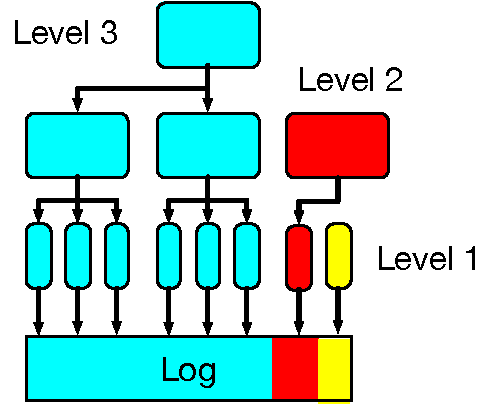
\includegraphics[height=0.5\textwidth]{figures/routing_tree.pdf}
		\caption{The routing trees in a 3 level BOT. The trees
                  cover contiguous portions of the log.  The highest
                  level covers the beginning of the log, the next
                  level the beginning of the remainder of the log, and so on.}
		\label{fig:routing_tree}
	\end{minipage}\hfill
	\begin{minipage}[t]{0.55\textwidth}
		\centering
		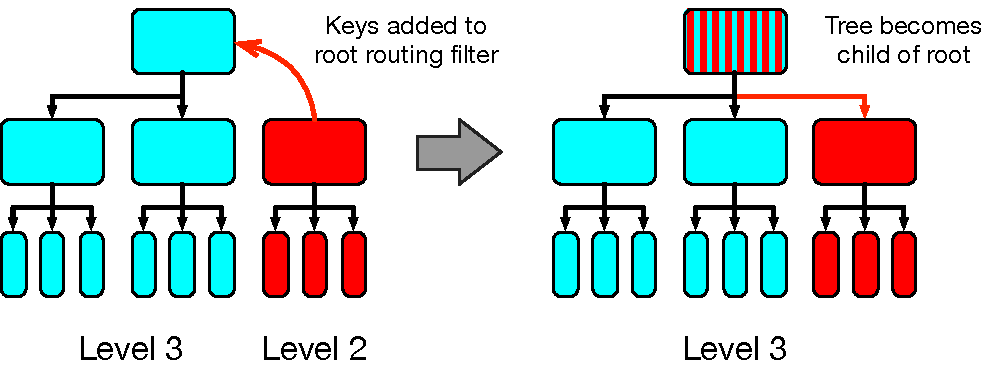
\includegraphics[height=0.4\textwidth]{figures/routing_tree_merge.pdf}
		\caption{When the routing tree on level $i$ fills, it is merged into
			the routing tree on level $i+1$. The now-full routing tree from
			level $i+1$ becomes a child of the root on level $i+1$. Its
			fingerprints are added to the root routing filter. Note that the
			tree is not moved.}
		\label{fig:routing_tree_merge}
	\end{minipage}
\end{figure}

When a level $i$ in the BOT fills, its routing tree is merged into the routing
tree of level $i+1$, thus increasing the degree of the target routing tree by 1 (and
perhaps filling level $i+1$, which triggers a merge of level $i+1$ into
$i+2$, and so on). The merge of level $i$ into level $i+1$ consists of adding
the prefix-sketch pairs of the fingerprints from level $i$ to the routing
filter of the root on level $i+1$. The child pointers of these pairs will point
to the root of the formerly level-$i$ routing tree, so it becomes a child of
the root of the level $i+1$ routing tree, although it isn't moved or copied.
See \Cref{fig:routing_tree_merge}. In this way, a BOT resembles an LT-LSM,
described in \Cref{sec:lsm}.

In order to add a fingerprint $K$ from level $i$ to the root routing filter on
level $i+1$, the prefix $P_{i+1}(K)$ must be known. However, the root routing
filter on level $i$ only stores the prefix $P_i(K)$ for each fingerprint $K$ it
contains, so that in particular the last character of $P_{i+1}(K)$ is missing.
As described in \Cref{sec:character-queue}, each level has a character queue,
which provides this character, as well as the check characters, in order to
merge the routing trees efficiently.

\subsection{Queries in a BOT}\label{sec:routing-tree-query}

A query to the BOT for a fingerprint $K$ is performed independently at each
level, beginning at the root of each routing tree. When a node is queried, its
routing filter returns a list of sketches. The sketches whose check characters
match the queried fingerprint indicate to which children the query is passed.
This process continues until the query reaches a block of the log, which is
then searched in full. In this way queries are ``routed'' down the tree on each
level to the part of log where the fingerprint and its associated value are.
Note that as queries descend the routing tree, they may generate false
positives which are likewise routed down towards the log.

In this section, we refine routing trees so that they offer two guarantees
about false positives. The first is that at each level, the probability that a
given false positive is not elinimated is at most $\frac{1}{\lambda}$. The
second is that false positives can only be created in the root, so that as the
query descends the tree, the number of false positives cannot increase.

During a query to a node of height $h$ for a fingerprint $K$, the routing
filter returns a list of sketches corresponding to fingerprints which match
$K$'s prefix. The query only proceeds on those children whose check characters
also match the check character $C_h(K)$. Since the characters of the
fingerprint are uniformly distributed and $\Theta(\log N)$-wise independent,
the check character of each false positive matches with probability
$\frac{1}{\lambda}$.  Moreover, the characters of each level are
non-overlapping, so for fingerprints $K$, $K'$ the event that $V_h(K)=V_h(K')$
is independent of the event that $V_{h-1}(K)=V_{h-1}(K')$.

To prevent new false positives from being generated when a query passes from a
parent to a child, the \defn{next character} of each fingerprint is also kept
in its sketch in the routing filter. For a fingerprint $K$ in a node of height
$h$, the next character is just the next character that follows the prefix,
$P_h(K)$, so that its prefix in the parent, $P_{h+1}(K)$, can be obtained. A
false positive in a child which is not in the parent will not match this next
character and can be eliminated.

When there are multiple prefix-matching fingerprints in both a parent and its
child, we would like to be able to align the lists returned by the routing
filters so that known false positives in the parent (either from check or next
characters) can be eliminated in the child. Otherwise the check character in
the child of a known false positive in the parent may match the queried
fingerprint, and therefore more than $\frac{1}{\lambda}$ of the false positives
may survive. To this end, we require the routing filter to return the list of
sketches in the order their fingerprint-value pairs appear in the log. Then
after the sketches in the child list whose next characters do not match the
parent are eliminated, the remaining phrases will be in the same order as in
the parent. In this way, known false positives can also be eliminated in the
child.

Now we can show:
\begin{lemma}\label[lemma]{lem:routing-tree-guarantee}
	During a query to a routing tree, the following are true:
	\begin{enumerate}
		\item A false positive can only be generated in the root.
		\item At each level, a given false positive survives with probability
			at most $\frac{1}{\lambda}$.
	\end{enumerate}
\end{lemma}

\begin{proof}
	Because of the next characters, false positives may only be created in the
	root of the routing tree. Each false positive in the root corresponds to a
	fingerprint $K'$ in the level. At each node on the path to $K'$'s location
	in the log, we use the ordering to determine which returned sketch
	corresponds to $K'$, so that the false positive corresponding to $K'$ is
	eliminated with probability $\frac{1}{\lambda}$.
\end{proof}


\subsection{Character Queue}\label{sec:character-queue}

The purpose of the character queue is to store all the sketches of fingerprints
contained in a level $i$ that will be needed during a merge in the future.
When level $i$ is merged into level $i+1$, the character queue outputs a sorted
list of the delta-encoded prefix-sketch pairs of all the fingerprints, which is
used to update the root routing tree. The character queue is then merged into
the character queue on level $i+1$.

The character queue effectively performs a merge sort on the sketches. If it
were to merge all the sketches as soon as they are available, this would
consist of $\lambda$-ary merges.  In order to increase the arity of the merges,
it defers merging sketches which are not needed immediately. The sketches are stored
collection of \defn{series}, by which we mean a collection of sorted runs. Each
series stores a continuous range of sketches
$S_i(K),S_{i+1}(K),\ldots,S_{i+j}(K)$ for each fingerprint $K$, together with
the prefix up to the first sketch, $P_{i-1}(K)$. These prefixes are delta
encoded in their run. Thus the size of an entry is determined by the number of
sketches in the range and the length of the prefix relative to the size of the
run (by \Cref{lem:delta-encoding}).

\paragraph{The character queue tradeoff}
We are faced with the following tradeoff. If the character queue merges a
series frequently, the delta encoding is more efficient, which decreases the
cost of the merging. However the arity is lower, which increases it. The
character queue uses a merging schedule which balances this tradeoff and thus
achieves optimal insertions.

\paragraph{The character queue merging schedule}
The character queue on level $i$ (here we consider blocks of the log to be
level $0$) contains the sketches $S_{i+1}(K), S_{i+2}(K),\ldots S_s(K)$ of each
fingerprint $K$ in the level. These characters are stored in a collection of
series $\{\sigma_{j_q}\}$, where $j_q$ is the smallest multiple of $2^q$
greater than $i$. Series $\sigma_{j_q}$ contains the sketches
$S_{j_q}(K),\ldots,S_{j_{q+1}-1}(K)$. Each series consists of a collection of
sorted runs each of which stores the delta encoded prefix of each fingerprint
together with its sketches.

Initially, when a block of the log is written, all the series $\sigma_{2^q}$
for $q=1,2,3,\ldots$ are created. When level $i$ fills, the runs in the series
$\sigma_{i+1}$ are merged, and the character queue outputs the delta encoded
prefix-sketch pairs, $(P_{i+1}(K),S_{i+1}(K))$ to update the root routing
filter on level $i+1$. If $2^{\rho(i+q)}$ is the greatest power of 2 dividing
$i+1$ ($\rho$ is sometimes referred to as the \defn{ruler
function}~\cite{wiki:Thomae's_function}), then $\sigma_{i+1}$ also contains the
next $2^{\rho(i+1)}-1$ sketches of each fingerprint. These are batched and
delta encoded to become runs in the series $\sigma_{j_q}$ for $q =
[0,\rho(i+1)]$. The runs in the remaining series of level $i$ becomes runs of
their respective series on level $i+1$.

Note that for the lower levels, some runs may be shorter than $B$ due to the
delta encoding. For a run in a series $\sigma_q$, this is handled by buffering
them with the runs $\sigma_q$ of higher levels and writing them out once they
are of size $B$. Note that this requires $O(B\log\log N)$ memory.

This leads to the following merging pattern: $\sigma_j$ batches $2^{\rho(j)}$
sketches, and has delta encoded prefixes of $2^{\rho(j)}$ characters on average,
by \Cref{lem:delta-encoding}. Therefore,

\begin{lemma}\label[lemma]{lem:character-queue-size}
	A series $\sigma_j$ in a character queue contains $O(2^{\rho(j)})$
	characters per fingerprint.
\end{lemma}

This leads to a merging schedule where the characters per item merged on the
$j$th level is $O(2^{\rho(j)})$. Starting from 1 this is
$1,2,1,4,1,2,1,8,1,2,1,4,1,2,1,16,\ldots$, which resemble the tick marks of a
ruler, hence the name ruler function.

We now analyze the cost of maintaining the character queues.

\begin{lemma}\label[lemma]{lem:character-queue-update}
	The total per-insertion/deletion cost to update the character queues in a
	BOT is $\Theta\left(\frac{1}{B}\left(\log_{\frac{M}{B}} N + \log\log
	M\right)\right)$.
\end{lemma}

\begin{proof}
	When $\sigma_j$ is merged, $\lambda^{2^\rho(j)}$ runs are merged, which has
	a cost of
	$O\left(\frac{2^{\rho(j)}}{B}\left\lceil\log_{M/B}\left(\lambda^{2^\rho(j)}\right)\right\rceil\right)$
	characters per fingerprint.

	There are $\log_\lambda \frac{N}{B} = O(\log_\lambda N)$ levels, so this leads to the
	following total cost in terms of characters:

	\begin{align*}
		O\left(\sum_{i=1}^{\log_\lambda N} 2^{\rho(j)}\left\lceil\log_{\frac{M}{B}}\left(\lambda^{2^\rho(j)}\right)\right\rceil\right)
		&= O\left(\sum_{k=0}^{\log \log_\lambda N} \frac{\log_\lambda N}{2^k} \cdot 2^k \left\lceil\log_{\frac{M}{B}}\left(\lambda^{2^k}\right)\right\rceil\right) \\
		&= O\left(\log_\lambda N \left(\log\log M + \sum_{k=\log\log M}^{\log \log_\lambda N} 2^k\log_{\frac{M}{B}}\lambda\right)\right) \\
		&= O\left(\log_\lambda N\left(\log\log M + \log_{\frac{M}{B}}N\right)\right),
	\end{align*}
	where the last equality is because the RHS sum is dominated by its last
	term. Because there are $\log_\lambda N$ characters in a word, and all
	reads and writes are performed sequentially in runs of size at lease $B$,
	the result follows.
\end{proof}

\subsection{Performance of the BOT}

We can now prove Theorem 3:

\botcost*

\begin{proof}
	By \Cref{lem:refined-routing-filter}, the cost of updating the routing
	filters is $O\left(\frac{\grow}{B}\right)$, since there are $O(\log_\grow
	N)$ levels. This, together with the cost of updating the character queues,
	given by \Cref{lem:character-queue-update}, is the insertion cost.

	By \Cref{lem:routing-tree-guarantee}, a query for fingerprint $K$ on level
	$i$ incurs $O\left(\frac{1}{\lambda}\right)$ false positives in the root,
	and $O(1)$ nodes are accessed along each of their root-to-leaf paths. By
	\Cref{lem:refined-routing-filter}, each false positive thus incurs $O(D_K)$
	IOs.

	There are an expected $O\left(\frac{\log_\lambda N}{\lambda}\right)$ false
	positives across all levels, so, using \Cref{lem:chernoff} with
	$\delta=\lambda$, $O(D_K\log_\lambda N)$ nodes are accessed due to false
	positives w.h.p. For each time $K$ appears in the BOT, $O(\log_\lambda N)$
	nodes are accessed on its root-to-leaf path. By
	\Cref{lem:refined-routing-filter} the node accesses along each path incur
	$O(D_K\log_\lambda)$ IOs w.h.p., so accessing the nodes incurs
	$O(\log_\lambda N)$ IOs w.h.p.

	A block of the log is scanned at most $D_K$ times for true positives and
	also whenever a false positive from the level-$i$ root survives $i$ times.
	The expected number of such false positives for level $i$ is $1/\grow^i$,
	so the expected number across levels is $O\left(\frac{1}{\lambda}\right)$.
	Therefore by \Cref{lem:chernoff}, the number of blocks scanned is
	$O(D_K\log_\lambda N)$ w.h.p.
\end{proof}

\begin{corollary}\label[corollary]{cor:bot}
	Let $\mathcal{B}$ be a BOT with growth factor $\lambda$
	containing $N$ entries. If $\lambda = \Omega\left(\log_{\frac{M}{B}} N +
	\log\log M\right)$, then $\mathcal{B}$ is an optimal dictionary.
\end{corollary}
